\documentclass[11pt]{article}
\usepackage{acl2014}
\usepackage[utf8]{inputenc}
\usepackage{times}
\usepackage{url}
\usepackage{amsmath}
\usepackage[natbib=true,backend=bibtex,style=authoryear,language=english]{biblatex}
\usepackage{lipsum}
\usepackage{latexsym}
\usepackage[normalem]{ulem}
\usepackage[ruled]{algorithm2e}
\usepackage[]{setspace}
\useunder{\uline}{\ul}{}
\usepackage{caption} 
\usepackage{lastpage}
\usepackage{float}
\usepackage[page]{appendix}
\pagestyle{plain} 
\usepackage{graphicx}
\captionsetup[table]{skip=10pt}
\title{Comparing Traffic Control Strategies under Varying Conditions}

\addbibresource{references.bib}
\AtBeginBibliography{\small}

\author{Thomas van den Broek, Vincent Van Driel, Zsolt Harsányi, Tonio Weidler\\
	Department of Data Science \& Knowledge Engineering\\
	Maastricht, The Netherlands\\
	\tt \small vincevandriel@gmail.com, thomasbuo@gmail.com,\\
	\tt \small zsharsany@gmail.com, uni@tonioweidler.de
}
  
\begin{document}

\maketitle
\begin{abstract}
In this work, we create a traffic simulation evironment and apply various different contol strategies to try and optimize the flow of traffic. These strategies include changing the way the traffic lights cycle as well as changing various aspects of the roads, such as number of lanes and their types. We observed that different maps require different strategies and in some cases, only modifying the saturated roads help dissipate the traffic while traffic light control has little to no effect.

{{\it \bf Keywords:} traffic simulation; traffic control; strategies; linear programming; machine learning; realistic environment; IDM; MOBIL;}
\end{abstract}

\section{Introduction}
Intelligent traffic control systems attempt to regulate traffic in order to assure that all people reach their destinations in the most optimal time by minimizing their delay. These systems are important for the daily workings of major cities by alleviating traffic congestion and identifying problematic areas.

\subsection{Research Questions}
This work aims to evaluate various traffic control strategies and compare their effectiveness in different scenarios. In particular, we aim to investigate, whether different traffic signal control strategies are best suited for different street layouts, or if all maps induce consistent performance rankings. Furthermore, experiments are conducted in order to compare the effectiveness of strategies controlling the behaviour of traffic signals and such that are related to urban planning, e.g. introduction of new lanes or entirely new roads. We pose the question whether measures of urban planning can improve traffic beyond what was achieved by the best performing strategy.

\subsection{Approach}
Hence, in order to test the effect of different traffic control strategies, an appropriate simulation is required. For this purpose, we create a simulation environment which allows the incorporation of different such strategies into a dynamic traffic model. Our simulation aims to model the dynamics of a realistic environment as close as possible within the scope of the project, so that the comparison is meaningful and provides valuable data regarding the potential application of the strategies. 

The simulation is \textit{microscopic}. That is, instead of globally controlling traffic (\textit{macroscopic}), the atomic parts of the simulation are locally controlled cars \citep[see also][]{krajzewicz2002sumo}. Driving behaviour is modelled using the time- and space-continuous \textit{Intelligent Driver Model} (IDM) \citep{treiber2000congested}. 

We make our code publicly available at GitHub\footnote{https://github.com/weidler/traffic-simulation}.

\subsection{Related Work}
\label{sec:related-work}
In the following, previous research on this topic will be briefly summarized. Extensive work has been done on the simulation of traffic flow as well as the development of traffic control strategies. Following up on different approaches on modelling car following behaviour \citep[e.g.][]{gipps1981behavioural}, \citet{treiber2000congested} developed the influential \textit{Intelligent Driver Model} for the simulation of urban traffic. Similarly to the former, it creates a collision free environment where cars mind the  spacial and time-wise gap to the leading vehicle. The SUMO package \citep{krajzewicz2002sumo, behrisch2011sumo} utilizes the model by \citep{gipps1981behavioural} in an extended version \citep{krauss1998microscopic} in a complex simulation software. In contrast to their research, this work uses the IDM. Hence, the simulation is time-continuous, rather than time-discrete.

Often utilizing such simulation environments for evaluation purposes, a lot of research exists investigating the strengths of different approaches to the automatic control of traffic signals or traffic lights. \citet{papageorgiou2003review} have reviewed such research and identified two key characteristics according to which strategies may be classified. They distinguish between \textit{fixed-time} and \textit{traffic-responsive} strategies, as well as \textit{isolated} and \textit{coordinated} strategies. Fixed-time strategies use historical data to determine (e.g. by optimization) static cycle lengths, while traffic-responsive strategies may use different techniques (e.g. heuristics or optimization algorithms) in order to derive optimal cycle lengths from real-time data that has to be measured in some way. Isolated strategies are focused on a single intersection, while coordinated strategies are able to communicate information between multiple intersections and thereby make potentially joint decisions. \citet{coll2013linear} categorize strategies into four categories. They also distinguish between fixed-time and traffic-responsive approaches, but additionally differentiate \textit{adaptive systems} that apply optimization techniques and \textit{predictive strategies} that use both online and off-line information in order to predict future arrivals at the intersection \citep{coll2013linear}. In this work, the focus will be laid on the former two categories, that is, fixed-time and responsive.

There has also been research on more advanced strategies using e.g. different machine learning techniques like neural networks \citep[e.g.][]{srinivasan2006neural, chao2008intelligent} or linear programming \citep[e.g.][]{coll2013linear, lin2004enhanced} for optimizing the phase or cycle lengths of traffic lights. \citet[][]{coll2013linear} use predictions based on the queue size at red and green lights, flow capacity, and cycle length from the previous time step in order to optimize the cycle lengths with the help of linear programming. As the incoming traffic density from each road entering an intersection changes, the length of green and red phases for the corresponding traffic light is gradually adjusted to assure an optimal output flow. The objective function they optimize minimizes the queue lengths and maximizes the flow. 

\vspace{20pt}

In the following sections we further describe our approach and the results of our experiments. We begin by elaborating on the implementation of the simulation environment (section \ref{sec:envi}), followed by a description of different control strategies (section \ref{sec:strategies}). Following, the conducted experiments are described and the evaluation methodology is defined (section \ref{sec:experiments}). In section \ref{sec:results}, the results of these experiments will be reported. We conclude this work by discussing our results and proposing future directions.
	
\section{Simulation Environment}
\label{sec:envi}
In the following subsections we describe the implementation and design choices of the simulation environment in which we evaluated the effect of different traffic control strategies.
	
\subsection{Traffic Flow Simulation}
As mentioned beforehand, the IDM \citep{treiber2000congested} is applied for the simulation of car dynamics. It models traffic flow time- and space-continuous as a combination of \textit{free-road} and \textit{interaction} behaviour. The \textit{free-road term} is governed by a car's intention to reach its desired speed. The acceleration for this behaviour is calculated \citep{treiber2000congested} as

\begin{equation}
	\label{eq:free-road-term}
	\dot{v}_a^{\mathrm{free}}(t) = a ( 1 - ( \frac{v_a}{v_0} )^\delta),
\end{equation}

where $a$ refers to a cars maximum acceleration, $v_a$ is its current velocity and $v_0$ the desired velocity. When a car approaches a leading vehicle, it is supposed to slow down in order to avoid collision. This behaviour is modelled by an \textit{interaction term} which incorporates the distance to the leading vehicle and its speed \citep{treiber2000congested}. 

\begin{equation}
	\label{eq:int-term}
	\dot{v}_a^{\mathrm{int}}(t) = - a ( \frac{s_0 + v_a T}{s_a} + \frac{v_a \Delta v_a}{2 \sqrt{ab} s_a} )^2
\end{equation}

In the equation above, $s_0$ and $T$ restrict the car's minimum distance in space and time respectively. The interaction term will hence attenuate the free road term when approaching other cars, given by the complete equation for acceleration $\dot{v}(t)$

\begin{equation}
	\dot{v}(t) = \dot{v}_a^{\mathrm{free}}(t) + \dot{v}_a^{\mathrm{int}}(t)
\end{equation}

In order to simulate a time-continuous model, we need to numerically approximate the integration of the differential equations in \ref{eq:free-road-term} and \ref{eq:int-term}. For that, we choose a small time step $\Delta t$ and repetitively update the velocity as $v(t + \Delta t) = v(t) + \dot{v}(t)$.

\subsection{Traffic Rule Compliance}
Due to the large scale maps used in this work, drivers not only need to behave according to their own desires and other traffic participants. They additionally need to comply to a set of traffic rules as given by speed limits or traffic lights. Following, we briefly discuss the approaches we use in our simulation.

\paragraph{Approaching Traffic Lights} When approaching red traffic lights, drivers will stop in a predefined distance from the intersection, comparable to stop bars in real world streets. Cars that have already exceeded this line will drive through the intersection. 

\paragraph{Speed Limits} The IDM's free road term incorporates a driver's desired velocity as his intended maximum speed. We use an additional parameter, a driver's favoured velocity $v_{fav}$, and determine the desired velocity by taking the minimum of $v_{fav}$ and the roads speed limit.

\subsection{Lane Changing}
In order to incorporate lane changing behaviour into our traffic model, we apply the MOBIL model \citep{treiber2002realistische, kesting2007general}. MOBIL makes decisions for lane changing based on two questions: Is the lane change \textit{incentive} and is it \textit{safe}? The former question is answered based on the potential gain in acceleration on the new lane, while the latter decision is made based on the speed of and distance of the approaching car on the new lane.

\subsection{Arrival Times in a Continuous Simulation}
Rather than predefining arrival times for a fixed simulation duration, we dynamically generate inter-arrival times (IAT) during runtime. These IATs are drawn from a predefined distribution independently for each road in the map. Therefore, the amount of traffic on a map grows automatically with its size. We use a non-stationary poisson process based on real world data from the U.S. Department of Transportation \citep{trafficdata}. The hourly data is used to draw IATs based on a poisson process that is then adjusted using the thinning algorithm by \citet{lewis1979simulation}. The data used is shown in figure \ref{fig:traffic-data}. As can be observed, this creates rush hours around the hours of 7 to 9 am and 5 to 7 pm.

\begin{figure}[t]
	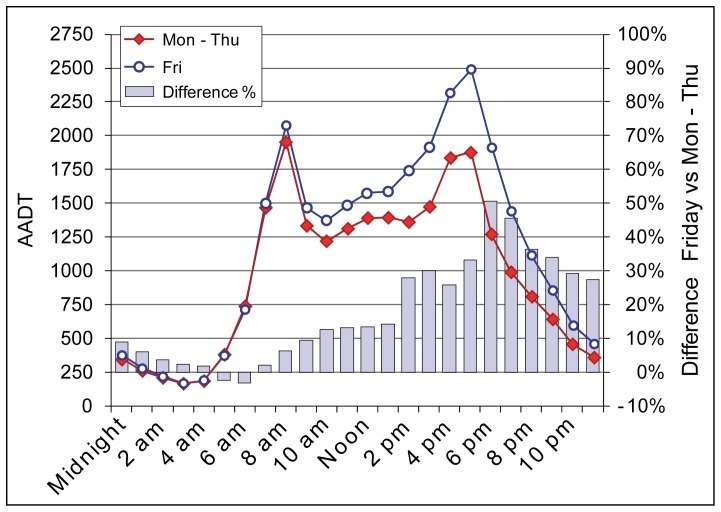
\includegraphics[width=\linewidth]{img/traffic-data.jpeg}
	\caption{Traffic data from the U.S. Department of Transportation. Graphic received from https://www.fhwa.dot.gov/policyinformation/tmguide/
	tmg\_2013/traffic-monitoring-methodologies.cfm \label{fig:traffic-data}}
\end{figure} 

\subsection{Population}
As \citet{papageorgiou2003review} state, most traffic signal strategies are only useful, when the roads are undersaturated with respect to traffic. For that reason but also for the sake of computational efficiency, the simulation prevents oversaturation by using a population count for each road. This population is initialized by determining how many cars would fit on the most outer lanes of that specific road. Cars will only spawn from roads as long as there is population available. Whenever a car leaves or arrives at a road, its population is respectively decremented or incremented.

\subsection{Zone-based Scheduling}
Aiming to increase the level of realism, roads on the simulated map have different types of zones that influence the spawn rates and routing of cars. Distinguished zones are \textit{residential}, \textit{mixed}, \textit{commercial} and \textit{industrial}. The zone type determines the traffic flow between different areas of the map. Based on the time of day, cars either mostly move from residential and mixed zones to industrial and commercial zone or vice versa, when they are on their way back home. This way, the simulation also incorporates the difficulties of heavy traffic in one direction, as faced in cities where living and working places are separated by its different areas. Figure \ref{fig:zone-traffic-flow} sketches how the traffic behaves between the zones based on the time of day.

\begin{figure}
	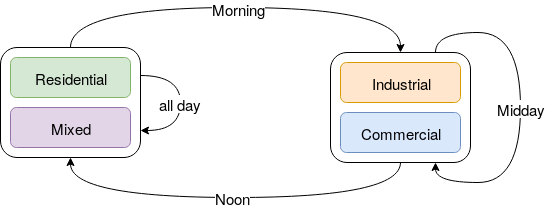
\includegraphics[width=\linewidth]{img/zoned-traffic-flow.png}
	\caption{Traffic Flow between different zone types at different times of the day. \label{fig:zone-traffic-flow}}
\end{figure}

\subsection{Path Finding}
Whenever a car enters the traffic, it needs to get a predefined route to take to its destination. In the simulation, each car runs an instance of a path finding algorithm, two of which were considered.

\paragraph{A*}
This popular path finding algorithm, based on Dijkstra’s algorithm \citep{dijkstra1959note}, was first introduced in 1968, by \citet{hart1968formal}. It finds the shortest path between the origin and the destination of the cars, given the map only taking the length of the path into account. This is done by using two scores for each node: H and G score. The H score is equal to the Euclidean distance from the node to the destination. The G score is the total distance travelled from the start node to the current node. Based on these two scores, the algorithm finds the shortest path between two points in a graph. 

\paragraph{Advanced A*}
The advanced A* path finding algorithm is very similar to the original version, but it also takes the traffic density and average speed of the roads into account. This is realized by calculating the traffic density and average speed of each road whenever the route of a car is created. The density of a road equals the number of cars on it divided by the length of the road, to get the number of cars per meter of road. The algorithm then adds a weighted density value to the G and H scores of the road to calculate the current best route. The average speed for the roads is taken from the continuously calculated statistics. The value of the average speed is subtracted from the score of the road, in order to incentivize the use of roads with a higher speed. Whith these modifications, the algorithm finds the fastest path instead of the shortest one.

Early experiments have shown that the advanced A* algorithm provides more safety against oversaturation of roads and therefore creates a more realistic simulation in which drivers are able to adjust their path based on their knowledge about the traffic.

\subsection{Simulation Model}
Putting the above parts together, the simulation procedure depicted by algorithm \ref{alg:simulation} is run.

\DontPrintSemicolon
\setstretch{1.2}
\begin{algorithm}[h]
	\;
	\KwData{Map m, CarList c, Schedule s, days d, delta\_t}
	\;
	\textit{Initialize} trafficlights\;
	\textit{Initialize} tracking variables\;
	\; 
	\While{simulated\_days $<$ d}{
		\textit{update} time\_parameters\;
		\;
		\ForEach{Road r in m}{
			\If{r.nextArrival == now}{
				\textit{spawn} car\;
				r.availablePopulation--\;
				\textit{generate} nextIAT\;
			}		
		}
		\;
		\textit{update} trafficlights\;
		\textit{update} car positions \textit{and} velocities\;
		\textit{remove} arrived\_cars \textit{and} adjust population\;
		\;
		\textit{visualize}\;
		\textit{track} statistics\;
	}
	\;
	\textit{report} statistics\;	
	
	\caption{Simulation procedure. \label{alg:simulation}}

\end{algorithm}
\setstretch{1}

\section{Traffic Control Strategies}

\begin{figure*}[htb]
	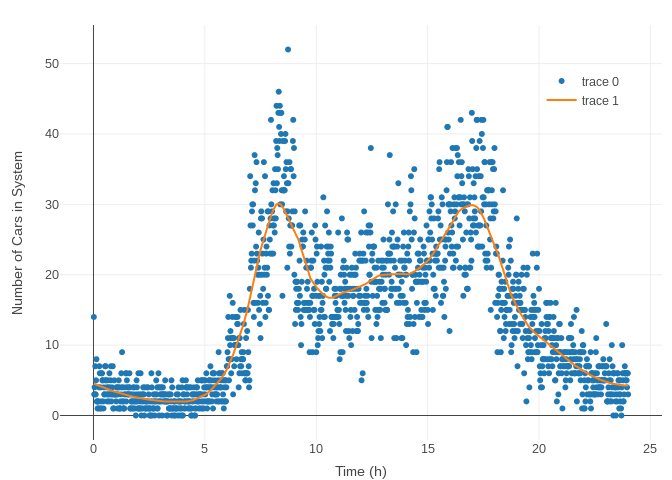
\includegraphics[width=0.33\textwidth]{img/number_of_cars_over_day.png}
	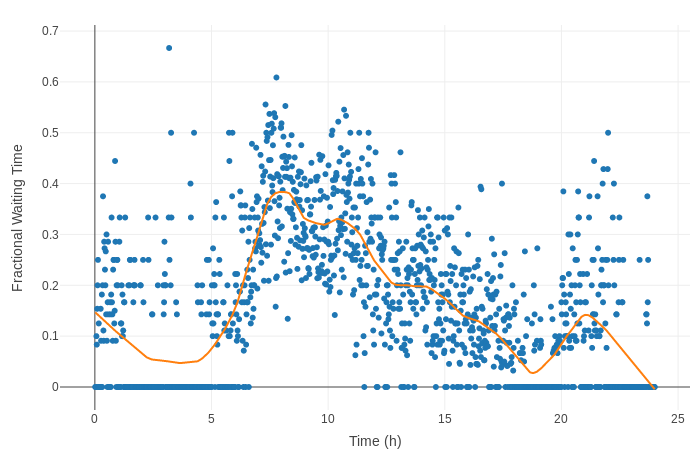
\includegraphics[width=0.33\textwidth]{img/velocity_over_day.png}
	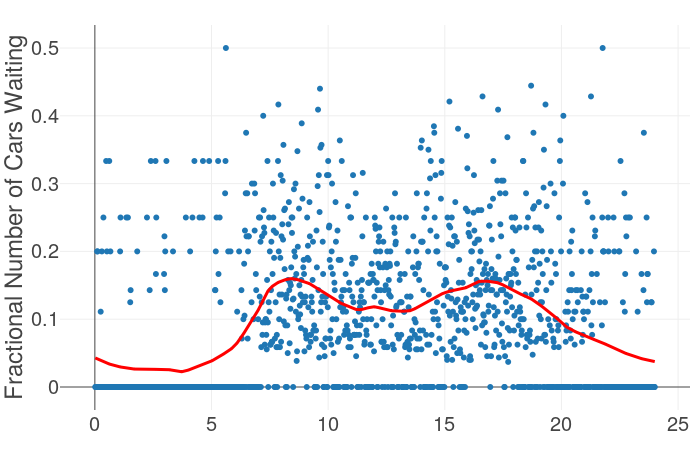
\includegraphics[width=0.33\textwidth]{img/frac_time_waitin.png}
	\caption{Number of cars (left), average velocity of cars (middle) and percentage of cars waiting (right) in the system simulated for one day. IATs are generated from the empirical distribution shown in figure \ref{fig:traffic-data}. \label{fig:validation}}
\end{figure*}

\label{sec:strategies}
In this section, the different traffic control strategies that will be compared in section \ref{sec:results} are described.

\subsection{Benchmark Strategies} 
In order to provide a baseline of what more advanced strategies should be able to outperform, two simple benchmark strategies were implemented. The first one is \textbf{Basic Cycling} and refers to a traffic light control strategy based on a simple, fixed-time cycle in which one traffic light at a time is green. The second one is \textbf{Informed Cycling} and refers to a similar strategy, in which a road's green phase is skipped if there are no cars waiting on it.

\subsection{Responsive Strategies}
\label{sec:responsive}
These methods mimic real-world examples of traffic control systems by acting similar to a traffic light with some form of traffic sensors (pressure plates, traffic cameras, etc.). 

Three strategies are investigated that, similarly to \textit{Basic Cycling}, choose the next green light in a given order. Crucially though, they do not use fixed times for the green phase. Instead, the phaselength is determined by some strategy-specific measure of traffic, normalised by the total traffic surrounding the intersection.

\paragraph{Density Weighted Cycling} The most simple of such strategies uses the total number of cars that come from a road to determine the phaselength of the traffic signal. It therefore assigns longer phaselengths to trafficlights that have more cars approaching the intersection relative to all other incoming roads.

\paragraph{Queue Weighted Cycling} Aiming to more precisely judge the severity of traffic load incoming from a road, this second weighting approach only takes into account cars that are actually waiting at a traffic light. A car is classified as waiting if it is slower than $5\ km/h$ and has a negative acceleration.

\paragraph{Flow Weighted Cycling} Finally, the last of such strategies weights by taking into account the traffic flow coming from a road during its previous green phase. Thereby, roads are preferred that predictively enqueue the most cars when turned green. The most apparent advantage of this approach is the fact that it will not give too much attention to overfilled roads that can actually not be relieved when lights turn green because the following traffic disallows it.

\vspace{20pt}
Dynamic strategies are strategies that instead of deciding how long a light has to stay green decides which light to turn green based on the information that the intersection gathers. Currently there are two strategies that do this.

\paragraph{Dynamic Cycling} The first strategy that determines which light of an intersection should turn green is Dynamic Cycling. This strategy measures the amount of cars that are moving towards the intersection for each connected road and chooses to turn the light green for the road which has the most incoming traffic. It makes the next decision at a set interval.

\paragraph{Dynamic Cycling+} The second strategy is Dynaminc Cycling+. This strategy is a more advanced version of the regular Dynamic Cycling. The differenc is that Dynamic Cycling+ does not only measure the incoming traffic for each road but also measures their average speed. it chooses to turn the light green for the road with the lowest average speed. Should the average speed of two or more roads be close to each other, then the intersection will choose the road with teh most incoming traffic. Another feature this strategy has is that at every traffic light has to turn green at least once within a certain amount of time. This is to prevent some roads from never turning green and thus causing some cars to never be able to drive.

\section{Methodology \& Experiments}
\label{sec:experiments}

\subsection{Simulated Maps}
Experiments are conducted on three different maps.They differ in the challenges that they impose on the traffic light systems and are therefore supposed to test their strengths and weaknesses. In the following, the three maps are described and motivated. Images can be found in the Appendix.

\paragraph{Two Districts} “Two Districts” is a small and simple map, designed to test the effects of modifying the most crucial roads in a map. The map has a residential district on the left and an industrial district on the right, connected by only one road, in order to force most vehicles to take it during the rush hours. This road is then modified in various ways, including adding lanes, changing it to a highway and also replaced by multiple one-way streets. 

\paragraph{Brusselsepoort} This map is modelled after a part of Maastricht called Brusselsepoort. It includes lots of residential areas, and a small commercial zone. This map was included in the testing as to have a “real world” scenario. This map was used to find the optimal phase lengths for the strategies.

\paragraph{Tie Fighter} The “Tie Fighter” map has three sections. In the middle, there is a residential area, spawning most of the traffic in the morning. The left and right side of the map are industrial and commercial areas. The three sections are connected by three lane highways. The map is not the most realistic, but it can be a challenging case for the traffic light strategies, due to the often-saturated mid-section.

\subsection{Simulation Validation}
In order to validate both the IA generation as well as the general behaviour of different measures and dynamics, we validated the simulation environment using the average speed of cars, their number on the map as well as fractional waiting times in the simulation as a development over one day. Figure \ref{fig:validation} shows the results in three graphs. As can be observed, not only the density, but also both other dependent measures resemble the rush hour pattern from the original data.

\subsection{Methodology}
In order to perform statistical calculations on the data, it is often necessary but at least useful to have IID observations. It is obvious that this independence can not be assumed in a traffic simulation between individual cars, since the delay of one car often influences that of others in shared roads and queues. While restarting the simulation $n$ times in order to get $n$ observations that can be combined to a grand mean seems an obvious choice, the day-based simulation also allows to run multiple days and assume independence between days, since traffic resets during night to a reasonable extend.

Since this is a non-terminating simulation, it is furthermore necessary to take a so called \textit{warm-up period} or \textit{transient phase} into account. It is the result of starting the simulation in an initial state that might not represent an actual state of the simulation in steady-state or inside a cycle. Therefore, the period where the simulation enters the steady-state needs to be removed from any statistical calculation such that it does not bias their results to the initial situation. Arguably, simulating traffic on the basis of days results in a cyclic simulation. Importantly though, this will not necessarily mean that the simulation entirely resets to zero cars in the system at midnight. For those reasons and the sake of convenience, in any experiment, the first simulated day will be removed from the simulation. 

It is the objective of this work to compare multiple systems (i.e. strategies) under different conditions. In order to rank these strategies, a convenient framework for such a comparison would be needed. An all-pairwise comparison is not desirable, since the total of 7 systems would require 30 comparisons, which would result in tiny confidence levels due to the Bonferroni inequality \citep[see e.g.][]{law2007simulation}. Instead, the sample size required for each system in order to achieve a confidence level of $\alpha$ for the complete ranking can be determined by the approach of \citet{dudewicz1975allocation}. Though, given the number of strategies to compare and the fact that we care about relatively small differences in the systems, fairly high numbers of simulated days would be necessary to guarantee a significant ranking with e.g. an significance level of $0.05$ (about 4000 days for e.g. flow weighted cycling). The computationally expensive simulation environment used in this work does not allow us to run such large experiments in feasible time. We therefore fall back to a comparison with benchmark strategies and report significance of the differences using paired t-confidence-intervals.

Two measures are employed to compare the performance strategies. Similarly to prior work \citep{srinivasan2006neural}, the average velocity of cars in the system is measured. Additionally, we report the percentage of cars waiting (as defined in section \ref{sec:responsive}) in order to measure general queue length.

\section{Results}
\label{sec:results}
In the following section, results for all experiments are presented. Firstly, the outcome of the optimization of the phase length parameter are reported and shortly discussed. Secondly, for each street layout, the performances of all strategies will be used to rank them. In the last subsection, the influence of some urban planning measures will be investigated.

\subsection{Phase Length Optimization}
Experiments for the optimization of phase lengths in all strategies were conducted on the Brusselsepoort map with 5 different configurations each and a simulation duration of 21 days (where the first day was removed as the transient phase. As the measure to be optimized on, we choose the average speed, since this is one of the most common metrics in the literature. Results of those experiments for the basic, informed and flow weighted strategy can be found in the appendix in figure \ref{fig:opt-results} in the form of box plots as an average during the rush hour between 7 and 9 o'clock.

In both Basic and Informed Cycling, 10 seconds and 25 seconds are respectively the best and second best performing strategies numerically. Since 10 seconds is a rather low phase length which might get its benefits from the specific design of the simulation environment, we choose 25 seconds as the phase length for these two strategies in the following experiments. For the Flow Weighted Cycling (and it will be assumed here, that this generalizes to the similar other responsive strategies) higher phase lengths induce worse performance. Again, for the sake of realism we choose a cycle length of 30 seconds and do not consider lower values.

\subsection{Relative Ranking of Strategies}
Using the phase lengths chosen in the above section, experiments for all strategies on all maps were conducted. Each experiments ran 51 days long, such that the final score is the average of 50 days after the removal of the transient phase. In the following, tables contain averages for the first rush hour. Numbers for the afternoon's rush hour can be found in the Appendix.

\begin{figure*}[t]
	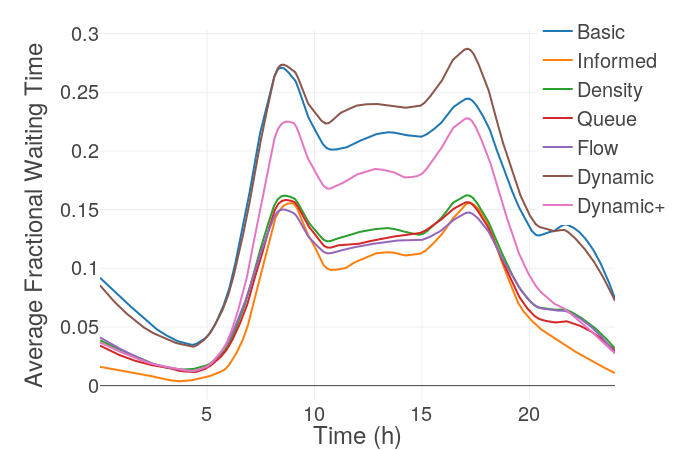
\includegraphics[width=0.33\textwidth]{img/frac_time_waiting_twodistr.png}
	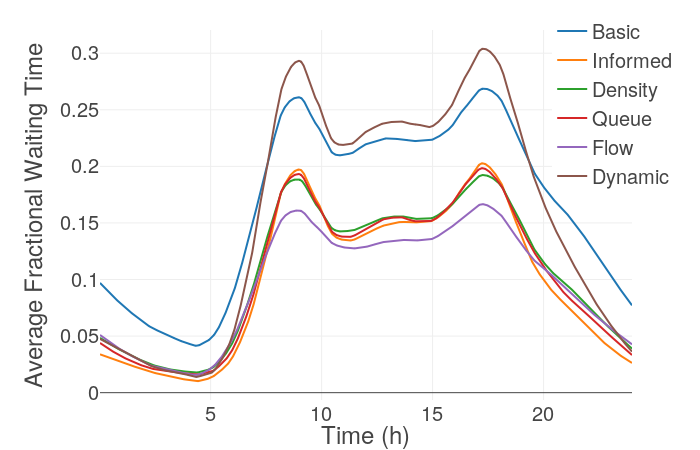
\includegraphics[width=0.33\textwidth]{img/frac_time_waiting_maas.png}
	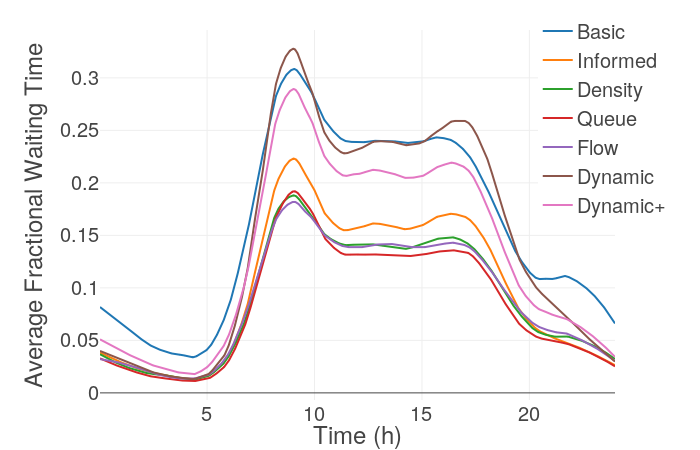
\includegraphics[width=0.33\textwidth]{img/frac_time_waiting_tie.png}
	\caption{Fraction of cars waiting in the experiments for Two-Districts (left), Brusselsepoort (middle) and the Tie-Fighter (right), as a development over a day. \label{fig:frac-waits-line}}
\end{figure*}

\begin{figure*}[t]
	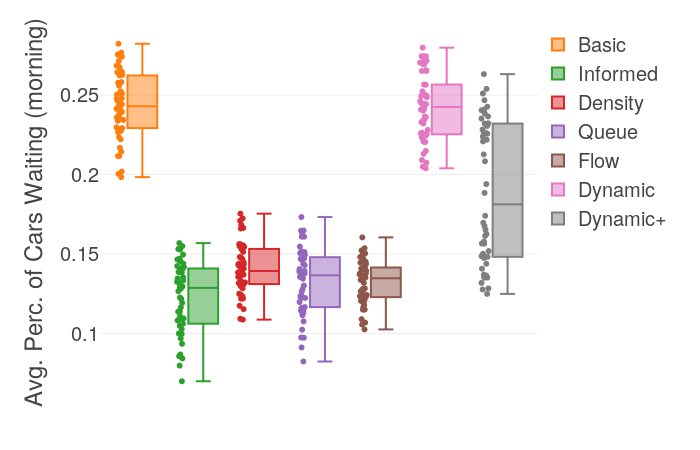
\includegraphics[width=0.33\textwidth]{img/frac_time_waiting_twodistr_bp.png}
	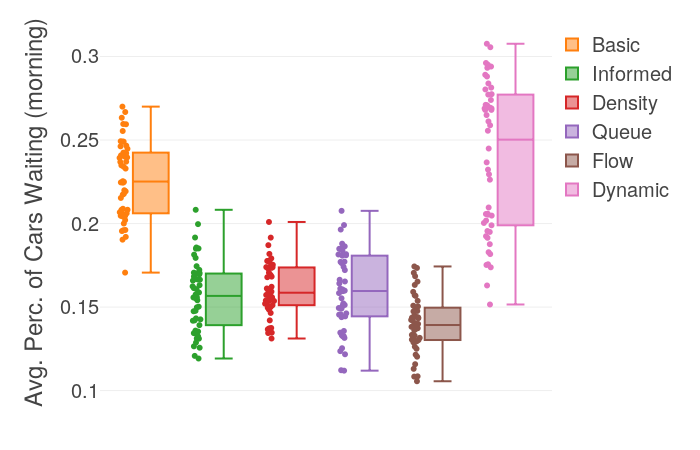
\includegraphics[width=0.33\textwidth]{img/frac_time_waiting_maas_bp.png}
	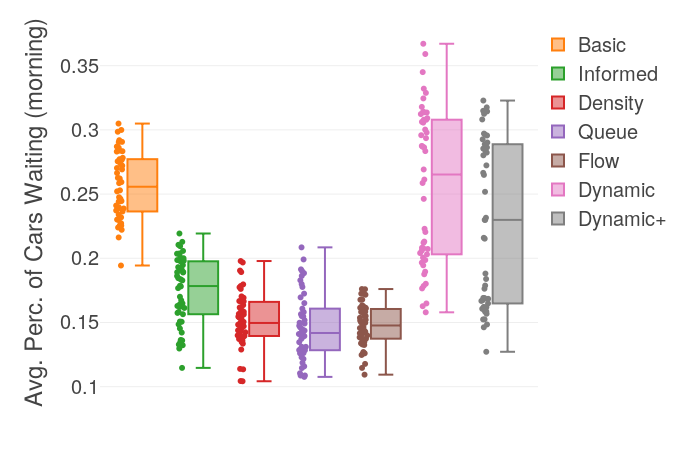
\includegraphics[width=0.33\textwidth]{img/frac_time_waiting_tie_bp.png}
	\caption{Fraction of cars waiting in the experiments for Two-Districts (left), Brusselsepoort (middle) and the Tie-Fighter (right) during morning rush hour as boxplots. \label{fig:frac-waits-bp}}
\end{figure*}

\subsection{Experiments on the Two-Districts Map}
\begin{table}[t]
\centering
\caption{Average Velocity of Cars during first rush hour (between 7am and 9am) on the Two-Districts map.}
\label{tab:velo-morning-twodi}
\begin{tabular}{l|l|l|l|}
\textbf{}                 & \textbf{Mean} & \textbf{$S^2(n)$} & \textbf{$S_{Means}^2(n)$} \\
\hline\textbf{Basic}      & 6.323          & 46.36             & 0.139                      \\
\textbf{Informed}   & \textbf{11.58}          & 133.15            & 0.596                      \\
\hline\textbf{Density W.} & 9.231*$^\dagger$          & 34.61             & 0.434                      \\
\textbf{Queue W.}   & 9.344*$^\dagger$ & 36.62             & 1.288                      \\
\textbf{Flow W.}    & 9.536*$^\dagger$          & 35.81             & 0.3752                     \\
\textbf{Dynamic}    & 6.015*$^\dagger$          & 36.75             & 0.0943                     \\
\textbf{Dynamic+}   & 2.461*$^\dagger$          & 8.5459            & 0.104                     
\end{tabular}
\vspace{20pt}
\centering
\caption{Fraction of Cars Waiting during first rush hour (between 7am and 9am) on the Two-District map.}
\label{tab:waiting-morning-twodi}
\begin{tabular}{l|l|l|l|}
\textbf{}                 & \textbf{Mean} & \textbf{$S^2(n)$} & \textbf{$S_{Means}^2(n)$} \\
\hline\textbf{Basic}      & 0.2435          & 0.017             & 0.0004                     \\
\textbf{Informed}   & \textbf{0.1229} & 0.0166            & 0.0004                     \\
\hline\textbf{Density W.} & 0.1409*$^\dagger$          & 0.014             & 0.0002                     \\
\textbf{Queue W.}   & 0.1332*$^\dagger$          & 0.0137            & 0.0004                     \\
\textbf{Flow W.}    & 0.1326*$^\dagger$      & 0.0139            & 0.0001                     \\
\textbf{Dynamic}    & 0.242$^\dagger$          & 0.242             & 0.0004                     \\
\textbf{Dynamic+}   & 0.189*$^\dagger$          & 0.0149             & 0.001                    
\end{tabular}

\small{* significant difference to basic, $^\dagger$ significant difference to informed}
\end{table}

On the first of three maps, the Informed cycling strategy outperforms all other strategies significantly in average velocity. Except for Dynamic and Dynamic+, all strategies outperform the Basic Cycling benchmark system, though. All results can be found in table \ref{tab:velo-morning-twodi}

With respect to the fraction of cars waiting (table \ref{tab:waiting-morning-twodi}), informed cycling is the best performing strategy again, but flow and queue weighted cycling are close runner-ups. All strategies but Dynamic Cycling can outperform the Basic Cylcing benchmark.

\subsection{Experiments on the Brusselsepoort Map}
On Brusselsepoort, Informed Cycling is significantly the best performing strategy for average speed, but is closely followed by Flow Weighted Cycling for average speed (see table \ref{tab:waiting-morning-brussel}. Dynamic Cycling again performs worst, and Dynamic+ even had to be terminated due to performance issues. Except for these two, all strategies can outperform Basic Cycling.

Measured in the fraction of waiting cars (table \ref{tab:waiting-morning-brussel}, Flow Weighted Cycling is the best performing system, significantly better than both Basic and Informed Cycling. Close runner-ups are Informed Cycling and Queue Weighted Cycling. As was observed before, all strategies except for the dynamic ones, outperform the Basic Cycling benchmark.

\begin{table}[H]
\centering
\caption{Average Velocity of Cars during first rush hour (between 7am and 9am) on the Brusselsepoort map.}
\label{tab:velo-morning-brussel}
\begin{tabular}{l|l|l|l|}
\textbf{}                 & \textbf{Mean} & \textbf{$S^2(n)$} & \textbf{$S_{Means}^2(n)$} \\
\hline\textbf{Basic}            & 6.34          & 41.65             & 0.064                      \\
\textbf{Informed}         & \textbf{9.86}          & 90.13             & 0.240                      \\
\hline\textbf{Density W.} & 8.46*$^\dagger$          & 20.80             & 0.304                      \\
\textbf{Queue W.}   & 7.55*$^\dagger$          & 20.07             & 0.649                      \\
\textbf{Flow W.}    & 9.00*$^\dagger$          & 23.02             & 0.239                      \\
\textbf{Dynamic}          & 1.99*$^\dagger$          & 3.997             & 0.073                      \\
\textbf{Dynamic+}         & -             & -                 & -                    
\end{tabular}
\vspace{20pt}
\centering
\caption{Fraction of Cars Waiting during first rush hour (between 7am and 9am) on the Brusselsepoort map.}
\label{tab:waiting-morning-brussel}
\begin{tabular}{l|l|l|l|}
\textbf{}                 & \textbf{Mean} & \textbf{$S^2(n)$} & \textbf{$S_{Means}^2(n)$} \\
\hline\textbf{Basic}      & 0.226          & 0.015             & 0.0005                     \\
\textbf{Informed}   & 0.156          & 0.017             & 0.0004                     \\
\hline\textbf{Density W.} & 0.1607*$^\dagger$         & 0.0119            & 0.0002                     \\
\textbf{Queue W.}   & 0.159*          & 0.0123            & 0.0005                     \\
\textbf{Flow W.}    & \textbf{0.139*$^\dagger$} & 0.010             & 0.0002                     \\
\textbf{Dynamic}    & 0.2387*$^\dagger$         & 0.0156            & 0.0019                     \\
\textbf{Dynamic+}   & -              & -                 & -                         
\end{tabular}

\small{* significant difference to basic, $^\dagger$ significant difference to informed}
\end{table}

\subsection{Experiments on the Tie-Fighter Map}
The Tie-Fighter map yields similar results to those of Brusselsepoort. The best-performing system measured in average speed (table \ref{tab:velo-morning-tie}) is Flow-Weighted Cycling, followed by Informed Cycling. Except for the dynamic strategies, all strategies significantly outperform Basic Cycling. The average fraction of cars waiting on this map (table \ref{tab:waiting-morning-tie} has its best score for Queue Weighted Cycling, but Flow Weighted Cycling follows with a difference of only 0.0008. For both measures, all systems except for the dynamic strategies outperform Basic Cycling significantly.

\begin{table}[h]
\centering
\caption{Average Velocity of Cars during first rush hour (between 7am and 9am) on the Tie-Fighter map.}
\label{tab:velo-morning-tie}
\begin{tabular}{l|l|l|l|}
\textbf{}                 & \textbf{Mean} & \textbf{$S^2(n)$} & \textbf{$S_{Means}^2(n)$} \\
\hline\textbf{Basic}            & 5.588          & 49.31             & 0.060                      \\
\textbf{Informed}         & 8.710          & 91.42             & 0.1881                     \\
\hline\textbf{Density W.} & 8.482*$^\dagger$          & 28.14             & 0.365                      \\
\textbf{Queue W.}   & 8.182*$^\dagger$          & 29.41             & 1.596                      \\
\textbf{Flow W.}    & \textbf{9.002*$^\dagger$} & 31.77             & 0.328                      \\
\textbf{Dynamic}          & 1.503*$^\dagger$          & 2.983             & 0.054                      \\
\textbf{Dynamic+}         & 1.574*$^\dagger$          & 3.251             & 0.078                   
\end{tabular}
\vspace{20pt}
\centering
\caption{Fraction of Cars Waiting during first rush hour (between 7am and 9am) on the Tie-Fighter map.}
\label{tab:waiting-morning-tie}
\begin{tabular}{l|l|l|l|}
\textbf{}                 & \textbf{Mean} & \textbf{$S^2(n)$} & \textbf{$S_{Means}^2(n)$} \\
\hline\textbf{Basic}      & 0.256           & 0.016             & 0.0006                     \\
\textbf{Informed}   & 0.1742          & 0.0215            & 0.0006                     \\
\hline\textbf{Density W.} & 0.1520*$^\dagger$          & 0.0127            & 0.0004                     \\
\textbf{Queue W.}   & \textbf{0.1467*$^\dagger$} & 0.0132            & 0.0006                     \\
\textbf{Flow W.}    & 0.1475$^\dagger$          & 0.01287           & 0.0002                     \\
\textbf{Dynamic}    & 0.2565*$^\dagger$          & 0.01699           & 0.0035                     \\
\textbf{Dynamic+}   & 0.2284*$^\dagger$          & 0.014             & 0.0040                    
\end{tabular}

\small{* significant difference to basic, $^\dagger$ significant difference to informed}
\end{table}

\vspace{20pt}

In figure \ref{fig:frac-waits-bp}, boxplots of the fractional number of cars waiting for the morning rush hour are shown. It becomes apparent that while the dynamic strategies are performing worse than other strategies with respect to the mean, they do also have large variance. In fact, the best results for those strategies even consistently outperform Basic Cycling.

\subsection{Urban Planning}
To investigate the effect of measures related to urban planning, three ways of changing the Two-Districts map were tested. Firstly, the number of lanes of the road connecting the districts was increased. Secondly, instead of one connecting road, multiple one-way roads were used to make moving from one district to the other possible. Finally, the connecting road is replaced by a highway. In all cases, Informed Cycling is the underlying traffic light strategy. Figure \ref{fig:urban-planning-stats} shows the results in the form of boxplots for the morning rush hour. All differences are significant with a significance level of $0.05$.

\begin{figure*}[t]
	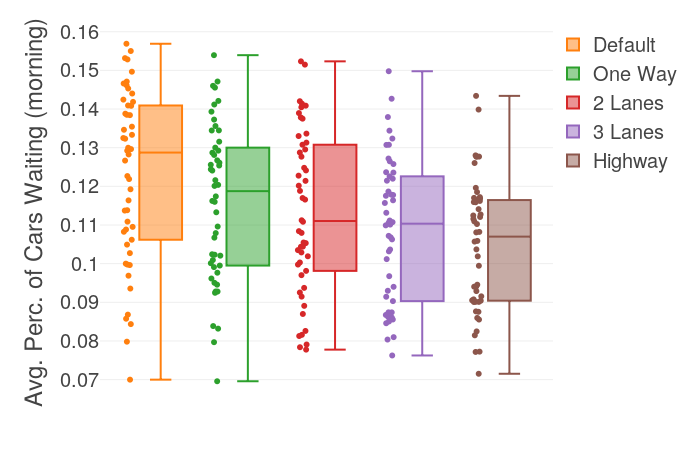
\includegraphics[width=0.5\textwidth]{img/urban_planning_frac.png}
	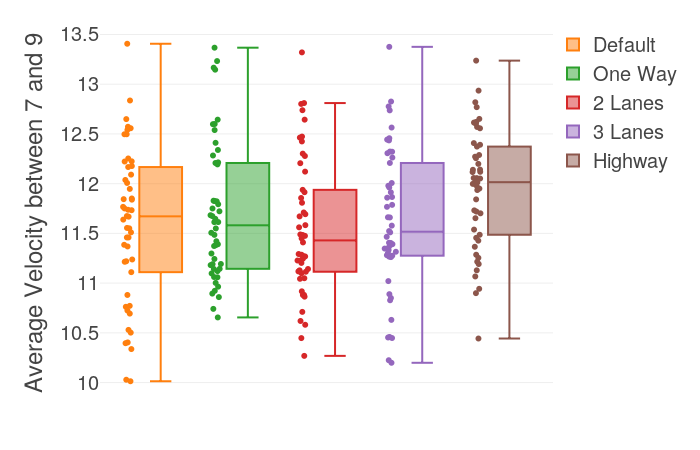
\includegraphics[width=0.5\textwidth]{img/urban_planning_velo.png}
	\caption{Fraction of cars waiting and average velocity for different map configurations in the form of boxplots. Default map is Two-Districts, the strategy used is informed cycling. \label{fig:urban-planning-stats}}
\end{figure*}

As can be observer, all measures improve the fraction of cars waiting. The smallest effect comes from one-way roads, while highways have the largest effect. There is no difference in the mean between two and three lanes, but for three lanes, the quantiles are shifted downwards. For the average velocity, only the introduction of a highway improved the result, while the other measures even slightly decrease the average velocity.

\section{Discussion}
\label{sec:discussion}
On the simple Two-Districts map, Informed Cycling is the best strategy by some margin. More complicated maps result in Flow and sometimes Queue Weighted Cycling to be superior, in particular when measured in fraction of cars waiting. This shows that the map design is an important factor for the choice of strategy. It can therefore not be assumed that there is a definite ranking in performance for such strategies. This implies for future work and the interpretation of prior research that the evaluation of strategies on single maps should be seen critically. It is advisable to always test strategies on a variety of maps that create different challenges. Furthermore, in real world application, city planners need to simulate specific intersections in order to decide for strategies per crossroad or area.

Throughout all experiments, informed cycling was a strong contender for the best strategy and even achieves this rank on the Two-Districts map. This shows that even simple heuristical strategies like the one at hand can achieve good results, improving performance vastly over Basic Cycling.

Interestingly, the weighted cycling strategies usually perform better when the measure of comparison is the percentage of cars waiting. Therefore, those strategies are more effective in minimizing queue length than in actually improving overall speed.

Dynamic+, even though it is the most adaptive strategy, does not perform well. Likely, this is caused by it always trying to resolve queues but in doing so it actually creates at least two new queues, depending on the number of roads connected to the intersection. This happens because the algorithm decides on which light to turn green based on the average speed and amount of cars on the road. However if for example we have an intersection with 4 connected roads and one road has a big queue, this road will continuously be selected as the traffic light that needs to be green. Unfortunately this causes the other roads to clutter up until they are weighted heavier that the currently most cluttered road. It was attempted to avoid this from happening by making every traffic light turn green once in a while but this impact was clearly not enough to counteract this problem.

\subsection{Future Work}
In future work, it could be promising to investigate more maps in order to identify exact road layouts that favour specific strategies. One hypothesis that the results on our maps for instance create, is that the grid-like layout of the Two-District map is a map type best suited for informed cycling. Furthermore, it should also be investigated whether our observations generalize to more advanced strategies using elaborate optimization techniques.

\section{Conclusion}
\label{sec:conclusion}
The results of three experiments on three different maps, ranking the 7 strategies used in this work, showed that different street layouts indeed induce different relative performances of the strategies. Furthermore, it was shown that when using one of the best performing strategies, changes to the street layout that relate to urban planning, can also be quite effective.

{\tiny\printbibliography}


\clearpage
\raggedbottom
\appendix
\begin{appendix}
\section{Maps}
\begin{figure}[h]
	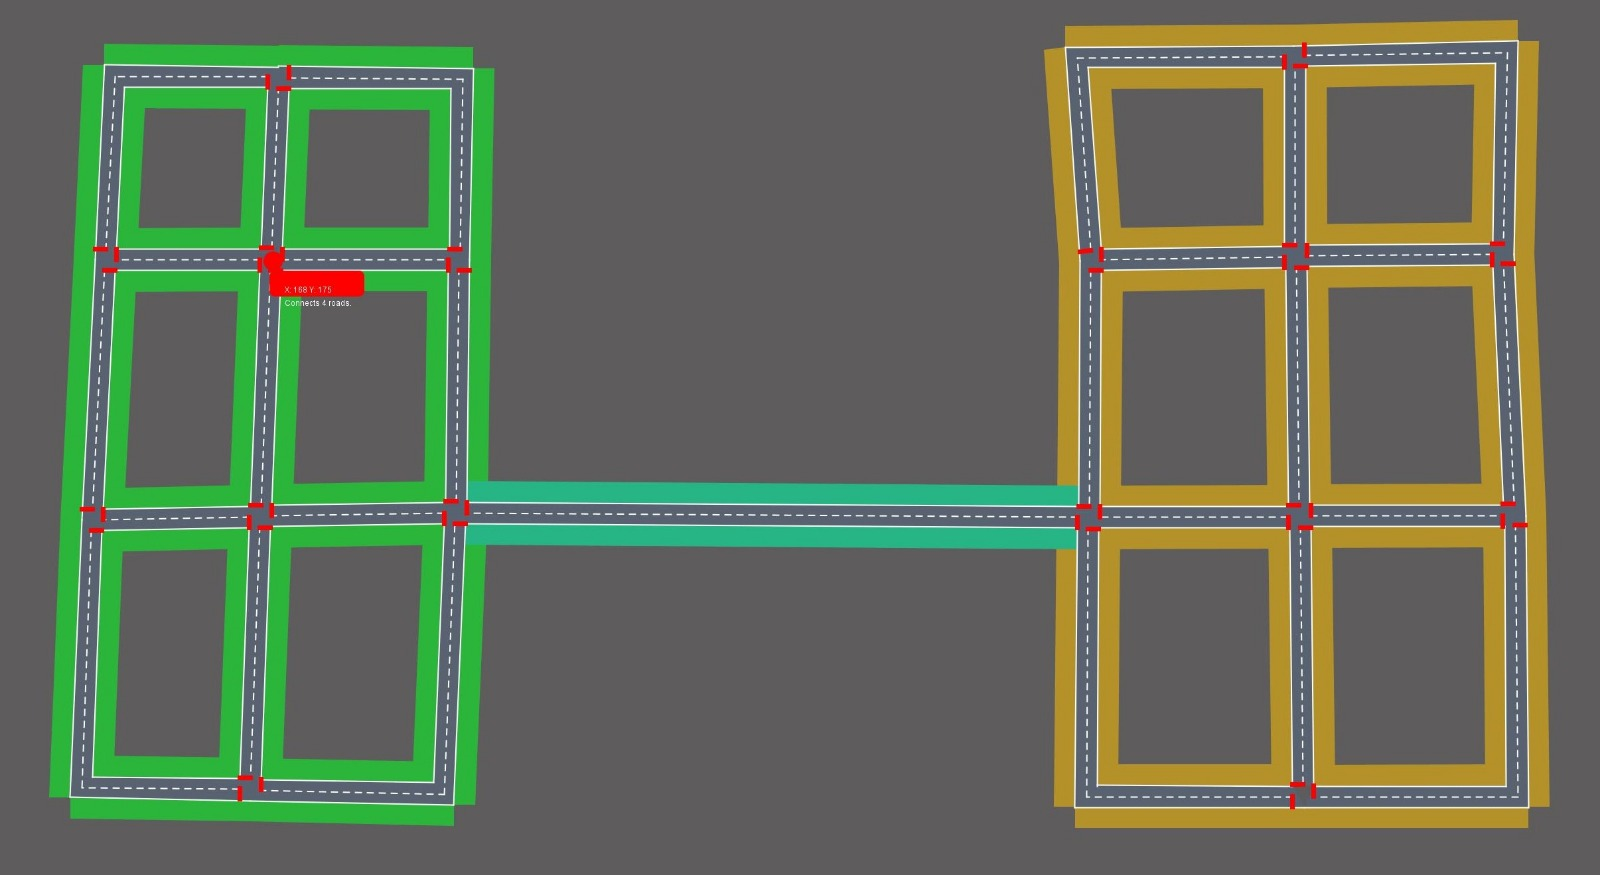
\includegraphics[width=\linewidth]{img/twodistr.jpeg}
	\caption{Map Two-Districts.}
\end{figure}

\begin{figure}[h]
	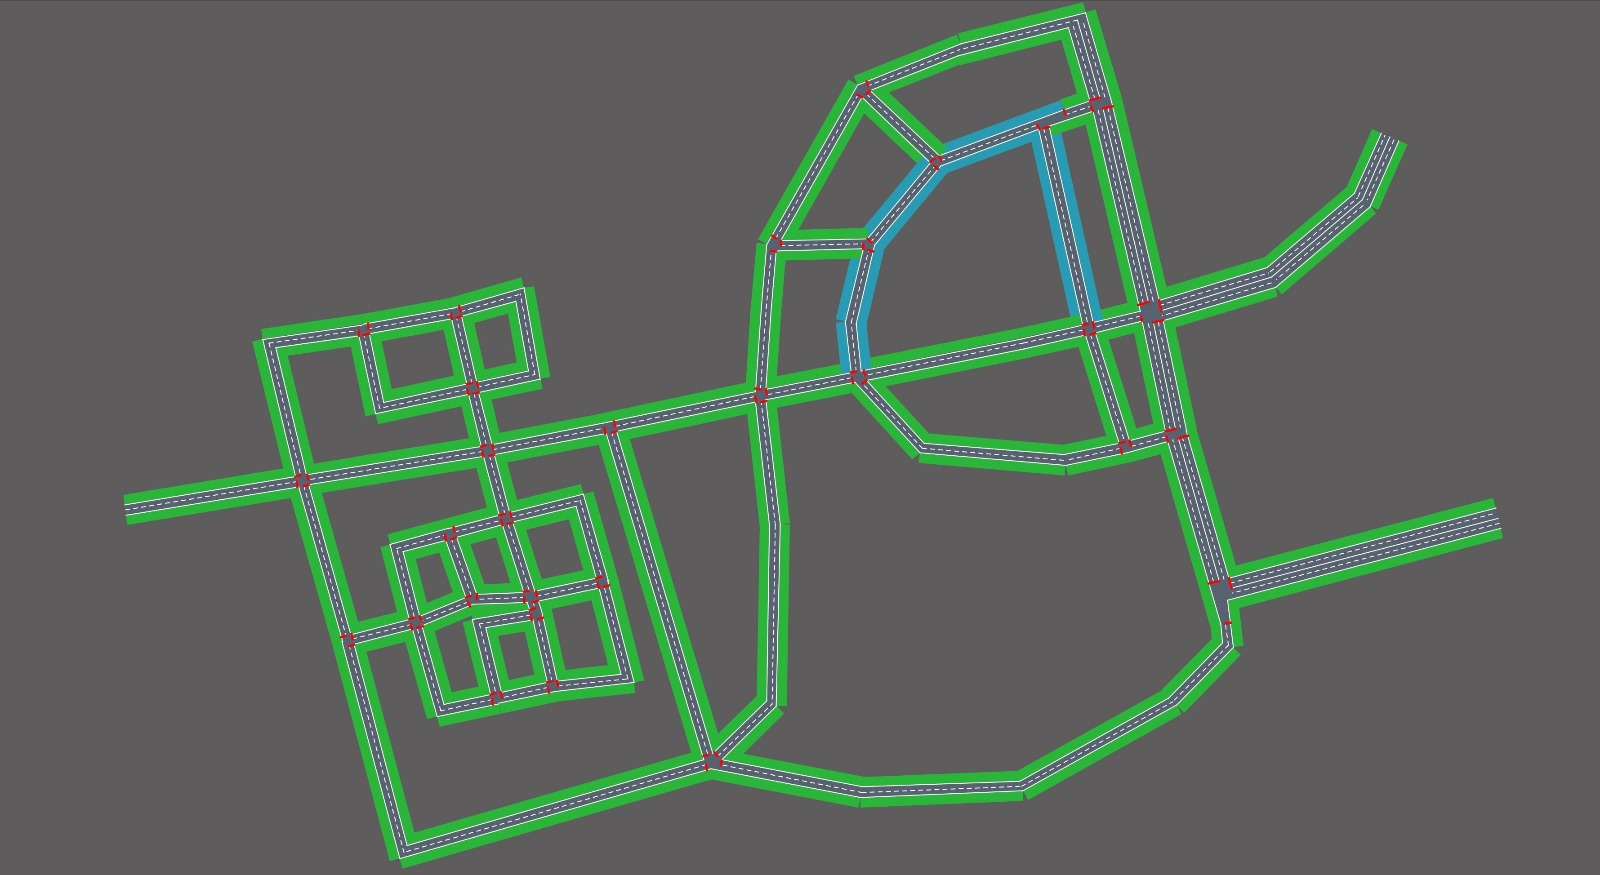
\includegraphics[width=\linewidth]{img/maas.jpeg}
	\caption{Map Brusselsepoort.}
\end{figure}

\begin{figure}[h]
	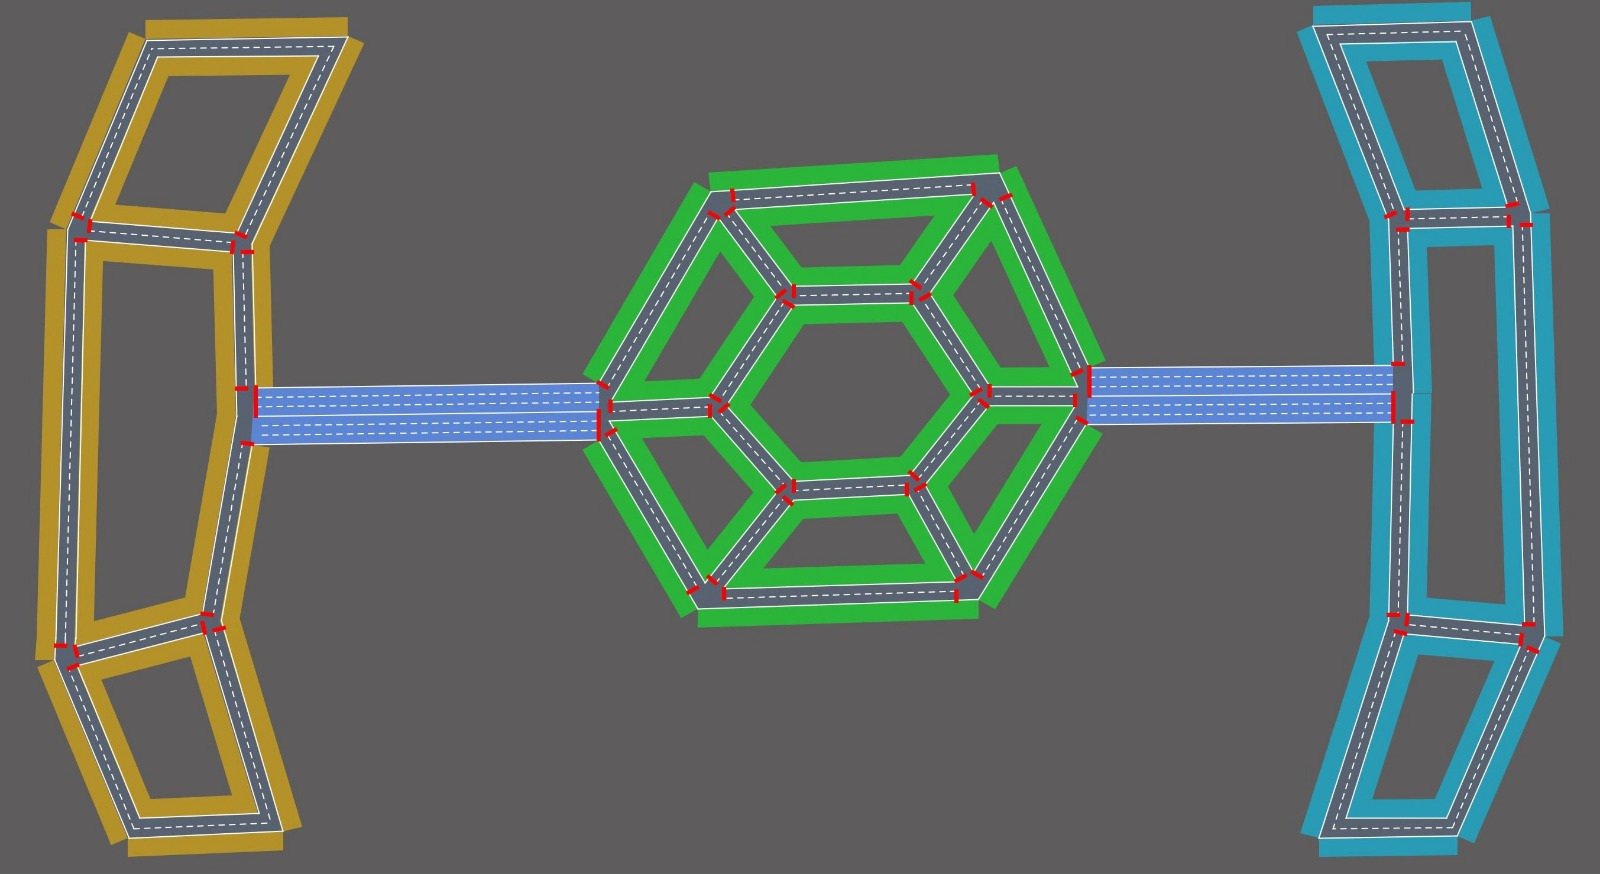
\includegraphics[width=\linewidth]{img/tie.jpeg}
	\caption{Map Tie-Fighter.}
\end{figure}

\clearpage
\section{Second Rush Hour Results}
\begin{table}[h]
\centering
\caption{Average Velocity of Cars during second rush hour (between 17am and 19am) on the Two-Districts map.}
\label{my-label}
\begin{tabular}{l|l|l|l|}
\textbf{}                 & \textbf{Mean} & \textbf{$S^2(n)$} & \textbf{$S_{Means}^2(n)$} \\
\hline\textbf{Basic}      & 6.900           & 43.806            & 0.06631                    \\
\textbf{Informed}   & \textbf{10.2690} & 106.758           & 0.2388                     \\
\hline\textbf{Density W.} & 8.9365*$^\dagger$           & 26.867            & 0.2742                     \\
\textbf{Queue W.}   & 8.902*$^\dagger$            & 28.91             & 0.811                      \\
\textbf{Flow W.}    & 9.105*$^\dagger$            & 28.58             & 0.2642                     \\
\textbf{Dynamic}    & 5.9756*$^\dagger$          & 27.924            & 0.0824                     \\
\textbf{Dynamic+}   & 9.9371*$^\dagger$           & 110.38            & 0.1399                    
\end{tabular}
\end{table}

\begin{table}[h]
\centering
\caption{Fraction of Cars Waiting during first rush hour (between 17am and 19am) on the Two-District map.}
\label{my-label}
\begin{tabular}{l|l|l|l|}
\textbf{}                 & \textbf{Mean} & \textbf{$S^2(n)$} & \textbf{$S_{Means}^2(n)$} \\
\hline\textbf{Basic}      & 0.221            & 0.012             & 0.0001                     \\
\textbf{Informed}   & 0.135            & 0.01492           & 0.0002                     \\
\hline\textbf{Density W.} & 0.1383*           & 0.0123            & 0.0001                     \\
\textbf{Queue W.}   & 0.1327*           & 0.0118            & 0.0001                     \\
\textbf{Flow W.}    & 0.1310*           & 0.0119            & 0.0001                     \\
\textbf{Dynamic}    & 0.252*$^\dagger$            & 0.0128            & 0.0002                     \\
\textbf{Dynamic+}   & \textbf{0.10620*$^\dagger$} & 0.0121            & 0.0000                    
\end{tabular}
\end{table}

\begin{table}[h]
\centering
\caption{Average Velocity of Cars during second rush hour (between 17am and 19am) on the Brusselsepoort map.}
\label{my-label}
\begin{tabular}{l|l|l|l|}
\textbf{}                 & \textbf{Mean} & \textbf{$S^2(n)$} & \textbf{$S_{Means}^2(n)$} \\
\hline\textbf{Basic}            & 6.190          & 33.74             & 0.040                      \\
\textbf{Informed}         & \textbf{9.524} & 74.75             & 0.156                      \\
\hline\textbf{Density W.} & 8.471*$^\dagger$          & 15.78             & 0.263                      \\
\textbf{Queue W.}   & 7.534*$^\dagger$          & 15.55             & 0.352                      \\
\textbf{Flow W.}    & 9.198*$^\dagger$          & 17.50             & 0.177                      \\
\textbf{Dynamic}          & 1.868*$^\dagger$          & 2.564             & 0.032                      \\
\textbf{Dynamic+}         & -              & -                 & -                         
\end{tabular}
\end{table}

\begin{table}[h]
\centering
\caption{Fraction of Cars Waiting during second rush hour (between 17am and 19am) on the Brusselsepoort map.}
\label{my-label}
\begin{tabular}{l|l|l|l|}
\textbf{}                 & \textbf{Mean} & \textbf{$S^2(n)$} & \textbf{$S_{Means}^2(n)$} \\
\hline\textbf{Basic}      & 0.2553         & 0.014             & 0.0001                     \\
\textbf{Informed}   & 0.182          & 0.016             & 0.0001                     \\
\hline\textbf{Density W.} & 0.1808*         & 0.0104            & 0.0001                     \\
\textbf{Queue W.}   & 0.1817*         & 0.011             & 0.0001                     \\
\textbf{Flow W.}    & \textbf{0.154*$^\dagger$} & 0.009             & 0.0001                     \\
\textbf{Dynamic}    & 0.2814*$^\dagger$         & 0.012             & 0.0001                     \\
\textbf{Dynamic+}   & -              & -                 & -                         
\end{tabular}
\end{table}

\begin{table}[h]
\centering
\caption{Average Velocity of Cars during first rush hour (between 17am and 19am) on the Tie-Fighter map.}
\label{my-label}
\begin{tabular}{l|l|l|l|}
\textbf{}                 & \textbf{Mean} & \textbf{$S^2(n)$} & \textbf{$S_{Means}^2(n)$} \\
\hline\textbf{Basic}            & 5.109          & 40.03             & 0.091                      \\
\textbf{Informed}         & 7.273          & 75.76             & 0.108                      \\
\hline\textbf{Density W.} & 7.481*$^\dagger$          & 22.69             & 0.295                      \\
\textbf{Queue W.}   & 7.803*$^\dagger$          & 23.47             & 1.735                      \\
\textbf{Flow W.}    & \textbf{7.826*$^\dagger$} & 23.13             & 0.261                      \\
\textbf{Dynamic}          & 1.399*$^\dagger$          & 1.932             & 0.030                      \\
\textbf{Dynamic+}         & 1.745*$^\dagger$         & 3.031             & 0.038                     
\end{tabular}
\end{table}

\begin{table}[h]
\centering
\caption{Fraction of Cars Waiting during second rush hour (between 17am and 19am) on the Tie-Fighter map.}
\label{my-label}
\begin{tabular}{l|l|l|l|}
\textbf{}                 & \textbf{Mean} & \textbf{$S^2(n)$} & \textbf{$S_{Means}^2(n)$} \\
\hline\textbf{Basic}      & 0.1934          & 0.0108            & 0.0001                     \\
\textbf{Informed}   & 0.1402          & 0.0140            & 0.0001                     \\
\hline\textbf{Density W.} & 0.1221*$^\dagger$          & 0.009             & 0.0001                     \\
\textbf{Queue W.}   & \textbf{0.1119*$^\dagger$} & 0.0094            & 0.0001                     \\
\textbf{Flow W.}    & 0.1202*$^\dagger$          & 0.010             & 0.0001                     \\
\textbf{Dynamic}    & 0.2193*$^\dagger$         & 0.0108            & 0.0001                     \\
\textbf{Dynamic+}   & 0.1762*$^\dagger$          & 0.0100            & 0.0001                    
\end{tabular}
\end{table}
\vfill
\clearpage
\section{Phase Length Optimization}
\begin{figure*}[h]
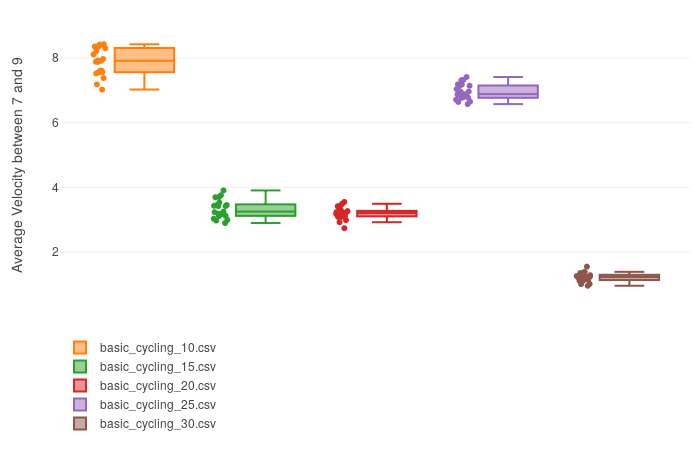
\includegraphics[width=0.5\textwidth]{img/basic-opt.png}
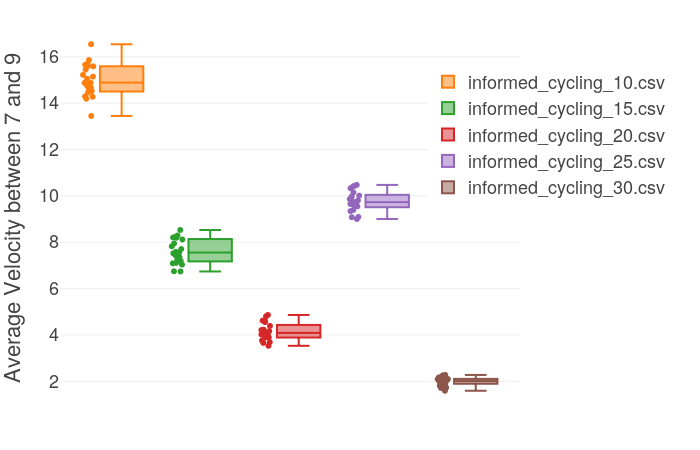
\includegraphics[width=0.5\textwidth]{img/informed-opt.png}
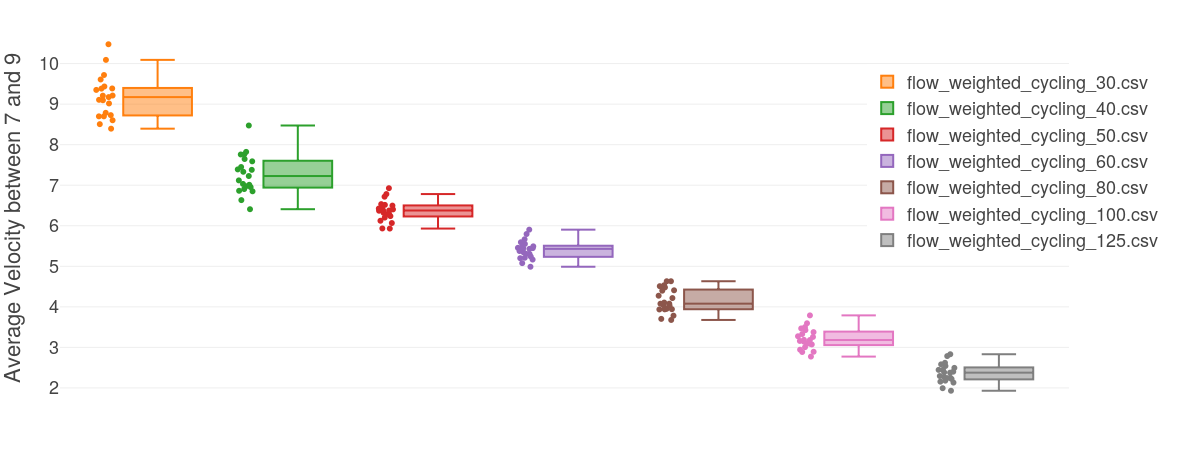
\includegraphics[width=\textwidth]{img/flow-opt.png}
\caption{Results for the phaselength optimization experiments for basic cycling, informed cycling and flow weighted cycling. \label{fig:opt-results}}
\end{figure*}

\end{appendix}


\end{document}